\documentclass[
    10pt,
    aspectratio=169,
    xcolor={dvipsnames},
    spanish,
    % handout,
    % notes=only,
    % notes,
    ]{beamer}

% BEAMER SETTINGS
\setbeamerfont{section in toc}{size=\normalsize, shape=\bfseries}
\mode<presentation>{
    \usetheme{Antibes}
    \setbeamercovered{transparent}
    \usecolortheme{rose}
    \setbeamertemplate{navigation symbols}{}
    }
\useoutertheme{infolines}

% PACKAGES
% \usepackage[spanish]{babel}  % uncomment for Spanish support
\usepackage{tikz,pgfplots}
\pgfplotsset{compat=1.13}
\usetikzlibrary{calc}

\usepackage{graphicx}
\graphicspath{{figures}}
\usepackage{booktabs}
\usepackage{upgreek}
\usepackage{commath}
\usepackage{amsmath,amsthm,amssymb,mathtools,mathrsfs}
\usepackage{cancel}
\usepackage{fontawesome5}
\usepackage{enumerate}
\usepackage{tensor}
\usepackage[font=footnotesize]{caption}
\usepackage{wasysym}

\usepackage[skins,theorems]{tcolorbox}
\tcbset{
    highlight math style={
        enhanced,
        coltext=black,
        colframe=black,
        colback=lightgray,
        arc=0pt,
        boxrule=.5pt
        }
}

% REFERENCES AND OTHERS
\usepackage{aas_macros}
\usepackage{natbib}
\bibpunct{(}{)}{;}{a}{}{,}

\usepackage{siunitx}
\sisetup{
    range-phrase=\text{--},
    range-units=single,
    separate-uncertainty=true,
    print-unity-mantissa=false
    }
\DeclareSIUnit{\gauss}{G}
\DeclareSIUnit{\jansky}{Jy}
\renewcommand{\figurename}{Fig.}

\usepackage{hyperref}
\hypersetup{
    % bookmarks=true,
    unicode=true,
    pdftoolbar=true,
    pdfmenubar=true,
    pdffitwindow=false,
    pdfstartview={FitH},
    pdftitle={Presentation},
    pdfauthor={Tomas Cassanelli},
    pdfcreator={Tomas Cassanelli},
    pdfnewwindow=true,
    colorlinks=true,
    linkcolor=RoyalBlue,
    citecolor=RoyalBlue,
    urlcolor=RoyalBlue
    }

\title[EL3103]{\bfseries Presentation title}
\subtitle{Presentation subtitle}
\author[Cassanelli]{Dr.~Tomás Cassanelli}
\institute[UChile]{Department of Electrical Engineering \\ Universidad de Chile}

\date{\today}

\begin{document}

\begin{frame}
  \titlepage
  \centering
  \faIcon{envelope} \href{mailto:tcassanelli@ing.uchile.cl}{tcassanelli@ing.uchile.cl} \hspace{.2cm}
\end{frame}

\begin{frame}
  \frametitle{Contenidos}
  \centering
  \begin{columns}
    \begin{column}{0.4\textwidth}
      \tableofcontents
    \end{column}
    \begin{column}{0.5\textwidth}
      \begin{figure}
        \centering
        
\includegraphics[width=\textwidth]{fcfm_die}
        \caption{Facultad de Ciencias Físicas y Matemáticas logo, Universidad de Chile.}
      \end{figure}
    \end{column}
  \end{columns}  
\end{frame}

\section{Introduction}

\begin{frame}
  \frametitle{Introduction}
  \begin{itemize}
    \item In beamer you define \texttt{frame}s to create a slide
    \item Each frame works similarly as a normal document in \LaTeX
    \item There are plenty of tutorials about it, find what fits you best! 
    \item The official documentation can be found here \url{https://ctan.org/pkg/beamer}
    \item A guide to the many styles is \href{https://web.mit.edu/rsi/www/pdfs/beamer-tutorial.pdf}{here}
  \end{itemize}
\end{frame}

\section{Blocks}

\begin{frame}
  \frametitle{Blocks and emphasis}
  \begin{block}{Theorem}
    You can create a \texttt{block} to put emphasis in a theorem or something else.
    \begin{equation*}
      \therefore e^{i\pi} + 1 = 0
    \end{equation*}
  \end{block}

  \begin{exampleblock}{Example}
    Similarly you can create a \texttt{exampleblock} for examples or interactive exercises.
    \begin{enumerate}
      \item This is the first question
      \item this is the second questions
    \end{enumerate}
  \end{exampleblock}

  \begin{alertblock}{Alert}
    This block is used to give an alert!
  \end{alertblock}
\end{frame}

\section{Citations}

\begin{frame}
  \frametitle{Citations}
  \centering
  \begin{columns}
    \begin{column}{0.4\textwidth}
      \begin{itemize}
        \item Citations are a \textbf{must}, and should always be cited with a citation command
        \item In the current example I am using \texttt{natbib} natural science style
        \item You can include other styles such as IEEE (which only supports \texttt{cite} command)
        \item To add a citation we use the \textit{natbib} package, which is the standard way of citation in natural sciences, a citation example would be like this \citep{2022A&A...663A.106C}
      \end{itemize}
    \end{column}
    \begin{column}{0.4\textwidth}
      \begin{itemize}
        \item The \texttt{natbib} in-line citations are:
        \begin{itemize}
            \item \citep{2022A&A...663A.106C}
            \item \citet{2022A&A...663A.106C}
            \item \citep[see][]{2022A&A...663A.106C}
        \end{itemize}
        \item You can also only quote the year or name using natbib:
        \begin{itemize}
          \item \citeyear{2022AJ....163...65C}
          \item \citealt{2022AJ....163...65C}
        \end{itemize}
      \end{itemize}
    \end{column}
  \end{columns}
\end{frame}

\section{Equations and units}

\begin{frame}
  \frametitle{Equations and units}
  \small
  \begin{itemize}
    \item When writing equations make sure you include the name of the variable in math mode and \textbf{not} in text mode, i.e., the variable is $z$ and \textbf{not} z, \textbf{z}, or \textit{z}
    \begin{equation}
      z = \sqrt{\del{\frac{x}{a}}^2 + \del{\frac{y}{b}}^2}
    \end{equation}
    \item You can highlight an important equation with the following command \texttt{tcbhighmath}
    \begin{equation}
      \tcbhighmath{\sigma_T \equiv k_c \frac{T_\text{sys}}{\sqrt{\Delta\nu t_\text{int}}}}
    \end{equation}
    \item I recommend using the \texttt{siunitx} package, to properly write units and numbers in \LaTeX, makes life so much easier, an example of this would be:
    \begin{equation}
        I_\nu\del{\nu,\widehat{\mathbf{n}}, \mathbf{r}, t}\dif\nu\dif\Omega \, \unit{\watt\per\m\squared}.
        \label{eq:specific_intensity}
    \end{equation}
    \item In Eq.~\eqref{eq:specific_intensity} we have added the units in math mode, they also work on text mode, e.g., \unit{\watt\per\m\squared}
    \item When defining a quantity use the \texttt{qty} command, same as in this example $c_0 = \qty{299792458.0}{\m\per\s}$
    \item For more about the units see the online documentation \url{https://ctan.org/pkg/siunitx}
  \end{itemize}
\end{frame}

\section{Tables}

\begin{frame}
  \frametitle{Tables}
  \centering
  \begin{columns}
    \begin{column}{0.5\textwidth}
      \begin{itemize}
        \item You may also be possible to include a Table, just make sure it is easy to read
        \item To make nice tables we suggest the package \texttt{booktabs}
        \item As shown in side Table, this lets you add bar lines and make the tables more compact
        \item Since it is a matter of taste feel free to look for your preferred one
      \end{itemize}
    \end{column}
    \begin{column}{0.4\textwidth}
      \begin{table}[t]
        \centering
        \begin{tabular}{ccc}
            \toprule
            \textbf{A} & \textbf{B} & \textbf{C} \\ \midrule
            1 & 2 & 3 \\
            1 & 2 & 3 \\
            1 & 2 & 3 \\
            1 & 2 & 3 \\
            1 & 2 & 3 \\
            \bottomrule
        \end{tabular}
        \caption{Adding a caption}
    \end{table}
    \end{column}
  \end{columns}  
\end{frame}

\section{Figures}
\subsection{Python}
\begin{frame}
  \frametitle{Python example figure}
  \begin{figure}
    \centering
    \includegraphics{planck.pdf}
    \caption{This is the Planck spectrum $B_\nu$. Notice that text matches the same one used in the presentation. You need to compile the figure within the \texttt{plot\_scripts/planck.py} directory. As a general rule, \textbf{always} include units in your plots.}
  \end{figure}
\end{frame}
\subsection{\texorpdfstring{Ti\textit{k}z}{Tikz}}
\begin{frame}
  \frametitle{Ti\textit{k}z example figure}
  \vspace{-.1cm}
  \begin{columns}
    \begin{column}[]{0.57\textwidth}
      \begin{figure}
        \centering
        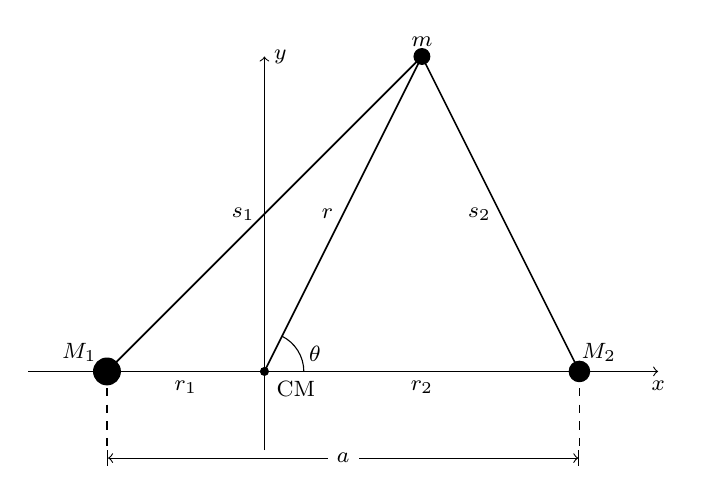
\begin{tikzpicture}[font=\footnotesize]
    
            \def\linethick{0.6pt}
    
            \coordinate (M1) at (-2, 0);
            \coordinate (m) at (2, 4);
            \coordinate (M2) at (4, 0);
    
            \draw[->] (-3, 0) -- (5, 0) node[left, below] {$x$};
            \draw[->] (0, -1) -- (0, 4) node[right] {$y$};
    
            \draw[line width=\linethick] (0, 0) -- node[midway,left] {$r$} (m) node[above] {$m$};
            \draw[line width=\linethick] (M1) node[above, xshift=-10] {$M_1$} -- node[midway,left] {$s_1$} (m);
            \draw[line width=\linethick] (M2) node[above, xshift=7] {$M_2$} -- node[midway,left] {$s_2$} (m);
    
            \path (M1) -- node[midway, below] {$r_1$} (0, 0);
            \path (0, 0) -- node[midway, below] {$r_2$} (M2);
    
            % Dashed lines
    
            \draw[dashed] (M1) -- ++ (0, -1);
            \draw[dashed] (M2) -- ++ (0, -1);
            \draw[|<->|] ($(M1) + (0, -1.1)$) -- node[midway,fill=white] {$a$} ($(M2) + (0, -1.1)$);
            
            \node[below] at (0.4, 0) {CM};
    
            \draw ([shift={(0, 0)}]64:0.5) arc[radius=0.5, start angle=64, end angle=0] node[above, xshift=4] {$\theta$};
    
            % balck circles
            \filldraw[black] (m) circle(0.1);
            \filldraw[black] (M1) circle(0.17);
            \filldraw[black] (M2) circle(0.13);
            \filldraw[black] (0, 0) circle(0.05);
    
        \end{tikzpicture}
        \caption{Nice diagram using Ti\textit{k}Z. Notice that the typesetting of variables is the same as the one used in \LaTeX. Variables $\theta$, $M_1$, $M_2$, have the same font and text style.}
        \label{fig:my_tikz_fig}
    \end{figure}
    \end{column}
    \begin{column}{0.43\textwidth}
      \begin{itemize}
        \item Remember to always reference all variables and labels within the figure
        \item The three body problem, with masses: $M_1, M_2,$ and $m$, etc.
        \item If you'd like to learn Ti\textit{k}z search online in \url{https://tex.stackexchange.com} there are already made examples that you can easily modify
        \item The official tutorial is here: \url{https://tikz.dev}
        \item \textbf{Warning} the learning curve for Ti\textit{k}z is super steep, but highly rewardable!
      \end{itemize}
    \end{column}
  \end{columns}

\end{frame}

\section{Conclusions}

\begin{frame}
  \frametitle{Conclusions}
  \begin{itemize}
    \item The summary/conclusions slide should reference all key points and takeaways of the talk
    \item End simple, with one or two conclusions
    \item Add a figure if needed
    \item Say thank you and open the door for questions
  \end{itemize}

  \vfill
  \begin{center}
    {\Large\textbf{Thank you!}}
  \end{center}

\end{frame}

\section{References}
\begin{frame}
    \frametitle{References}
    \footnotesize
    \bibliographystyle{bibstyle_aas}
    \bibliography{presentation_template.bib}
\end{frame}



\end{document}
